\chapter{Load-Flow Calculation}

\section{Problem Formulation}
The aim of an load-flow analysis is to determine the voltages in the power net. Any further information, like currents in connections, critically low voltages, etc. can be derived from this result. Therefore I will consider the problem to be solved if the voltages are known.
The first step in a load flow analysis is the modelling of the net elements, as it is way to complex to use a detailed description of for instance a power plant like \figref{power_plant}. Therefore, all elements in a power net are modelled through busses, also called nodes, and admittances between them.

\begin{figure}
	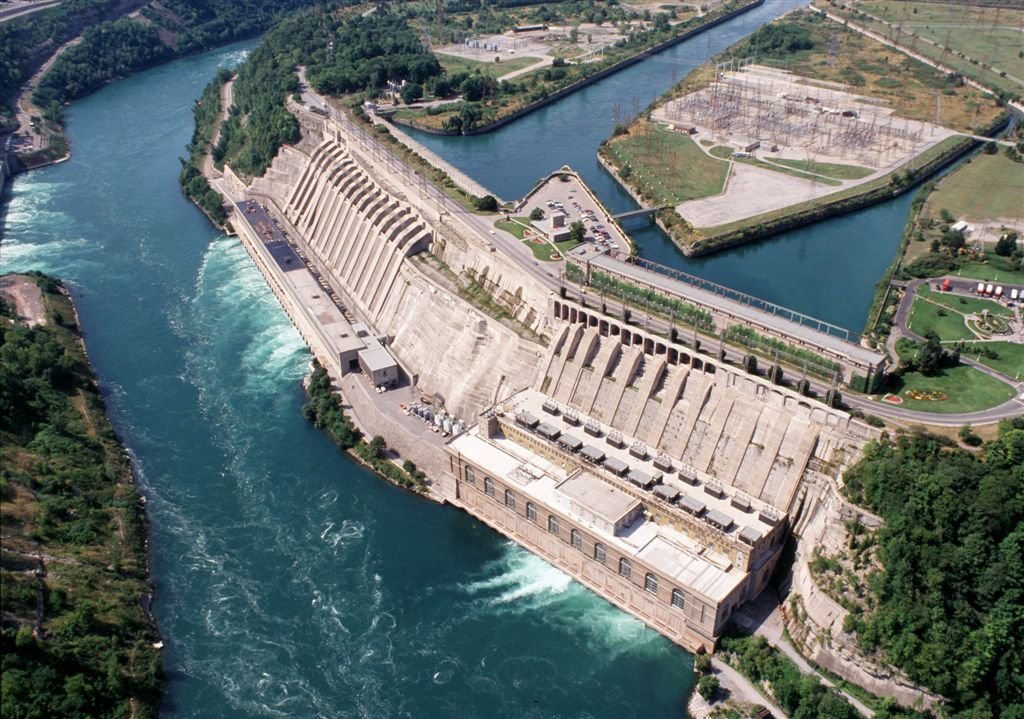
\includegraphics[width=\textwidth]{figures/adam_beck_complex.jpg}
	\caption{Sir Adam Beck Hydroelectric Generating Stations \cite{adam_back_complex}}
	\label{fig:power_plant}
\end{figure}

\subsection{Busses}
The most basic mathematical description of a an electric circuit, which an power net is, would be through admittances $Y_{ik}$ between the nodes $i$ and $k$, node voltages $U_k$ and branch currents $I_k$. In this case the element-based formulation
\begin{equation}
	\sum_i Y_{ik} U_i = I_k,
	\label{eq:current_controlled}
\end{equation}
will be used. If the loads and inputs would be current-controlled we could already stop at this point, solve the equation system and receive the node voltages as result. Unfortunately, most elements in a power net are defined through power, which is fed in, and load, which is drawn from the power net. Therefore, we have to extend \neweqref{current_controlled} with a term for a constant power $S_k = P_k + j Q_k = U_k I_k^\star$ at the node $k$ and receive
\begin{equation}
	\sum_i Y_{ik} U_i = I_k + \frac{S_j^\star}{U_j^\star}.
	\label{eq:pq_bus}
\end{equation}
This formula is already the definition of a so-called PQ-bus, as at the node the real and reactive power is the defined.
Another type of bus is a slack bus. At this bus the voltage is defined, therefore we do not need any further description of this bus, but the bus is also part from neighbour busses through the branch currents $Y_ik U_i$. In this case, if one of the branch currents is already known, this value can be moved to the right hand side of the equation \neweqref{pq_bus} and combined with $I_k$. Although, slack busses show up only in the constant currents of the right hand sides, there must be always at least one slack bus in the power net, as this bus then defines the rotation of the system and compensates mismatches in the total power sum. In practice, typically a major power plant is selected as slack bus.
The third important type of bus, beside the slack bus and PQ-bus, is the PV-bus. This is already some sort of control, as at such a node the real power $P_k$ and the voltage magnitude $|U_k|$ is defined. The implementation of this bus type depends on the algorithm which is used to calculate the missing node voltages, therefore I will discuss in the part about the different methods.

\subsection{Admittance Matrix}
The admittance matrix $\undertilde Y = (Y_{ik})$ is filled with the admittances between the nodes. More complex elements, like controlled sources, actually have to be voltage controlled, so that they can be modelled with an admittance matrix. Fortunately, most elements, which are not voltage controlled, can be transformed through a gyrator, which itself can be modelled through voltage controlled elements.

As during the modelling later several kinds of electric elements are used I will describe for each of them how they effect the admittance matrix.

\subsubsection{Admittance}

\subsubsection{Voltage Controlled Current Source}

\subsubsection{Gyrator}

\subsubsection{Current Controlled Current Source}

\subsubsection{Voltage Controlled Voltage Source}

\subsubsection{Ideal Transformer}

\section{Modelling of Net Elements}

The power net elements are modelled through admittances and busses, therefore we will use the previously derived knowledge to describe the behaviour of the net elements.

\subsection{Connection}
A connection is modelled only with admittances like in \figref{connection}. The values $Y_q$ and $Y_l$ can be derived from the physical properties of the connection through
\begin{equation}
	MISSING
\end{equation}
and
\begin{equation}
	MISSING.
\end{equation}

\begin{figure}
	\centering
	\begin{circuitikz}
	\draw (2, 0) to [R=$\frac{Y_{q}}{2}$,*-*] (2, 4);
	\draw (2, 4) to [R=$Y_{l}$,*-*] (6, 4);
	\draw (6, 0) to [R=$\frac{Y_{q}}{2}$,*-*] (6, 4);
	\draw (2, 0) to (6, 0);
	\draw (0, 0) to [short,*-*] (2, 0);
	\draw (0, 4) to [short,*-*] (2, 4);
	\draw (6, 0) to [short,*-*] (8, 0);
	\draw (6, 4) to [short,*-*] (8, 4);
	\draw (2, 0) to (2, -0.5) node[ground] {};
	\draw (0, 0) to [open,v^=$U_i$] (0, 4);
	\draw (8, 0) to [open,v=$U_j$] (8, 4);
\end{circuitikz} 

	\caption{Equivalent network of a connection}
	\label{fig:connection}
\end{figure}

\subsection{Load}

\subsection{Generator}

\subsection{Transformer}

\subsection{Feed-In}

\section{Calculation Methods}

\subsection{Classification of Methods}

\subsection{Current Iteration}
\label{sec:current_iteration}

\subsection{Newton-Raphson}
\label{sec:newton_raphson}

\subsection{Fast-decoupled-load-flow}
\label{sec:fdlf}

\subsection{Holomorphic Embedding Load Flow}
\label{sec:helm}

\subsubsection{Calculation of Coefficients}

\paragraph{Slack-Busses}

\paragraph{PQ-Busses}

\paragraph{PV-Busses}

\subsubsection{Analytic Continuation with Wynn's Epsilon Method}
